\documentclass{minimal}

\usepackage{tikz}
\usetikzlibrary{calc}
\usetikzlibrary{external}
\tikzexternalize[prefix=source/graphics/tikz/]

\usepackage[
    a4paper,
    margin=0pt,
    ignoreall
]{geometry}

\begin{document}
\tikzsetnextfilename{page-margin} % page margins
\noindent\begin{tikzpicture}
    \draw[line width=1pt] ($ (current page.north west)+( 1.5,-1.0) $) -- ++(-0.5,0) -- ++(0,-0.5);
    \draw[line width=1pt] ($ (current page.north east)+(-1.5,-1.0) $) -- ++( 0.5,0) -- ++(0,-0.5);
    \draw[line width=1pt] ($ (current page.south west)+( 1.5, 1.0) $) -- ++(-0.5,0) -- ++(0, 0.5);
    \draw[line width=1pt] ($ (current page.south east)+(-1.5, 1.0) $) -- ++( 0.5,0) -- ++(0, 0.5);
\end{tikzpicture}
\tikzsetnextfilename{binding-left} %left binding
\noindent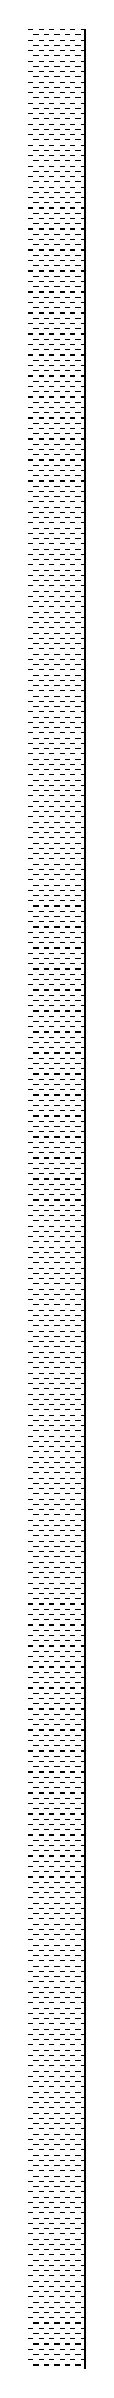
\begin{tikzpicture}[inner sep=0]
    % border
    \draw[line width=0.7pt] (0.72, +0.35pt) -- (0.72, -29.7cm-0.35pt);
    % dashes
    \foreach \y in {0,-0.1333,...,-29.6} {
        \draw[dash pattern=on 0.0667cm off 0.0667cm] (0, \y) -- ++(0.72, 0);
        \draw[dash pattern=on 0.0667cm off 0.0667cm, dash phase=0.0667cm] (0, \y-0.0667) -- ++(0.72, 0);
    }
\end{tikzpicture}
\tikzsetnextfilename{binding-right} %right binding
\noindent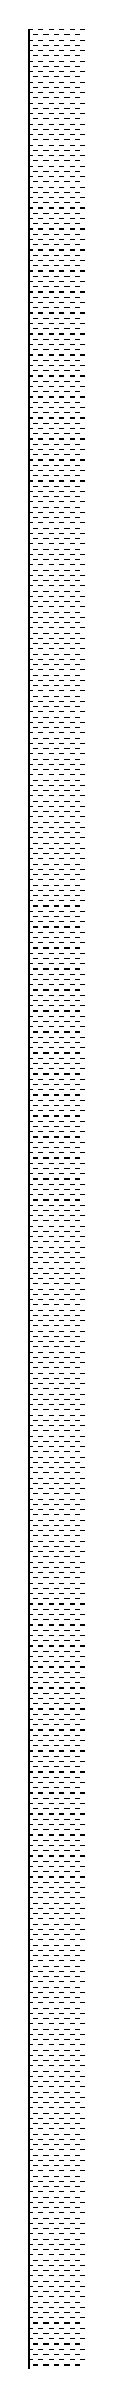
\begin{tikzpicture}
    % border
    \draw[line width=0.7pt] (-0.72, +0.35pt) -- (-0.72, -29.7cm-0.35pt);
    % dashes
    \foreach \y in {0,-0.1333,...,-29.6} {
        \draw[dash pattern=on 0.0667cm off 0.0667cm] (0, \y) -- ++(-0.72, 0);
        \draw[dash pattern=on 0.0667cm off 0.0667cm, dash phase=0.0667cm] (0, \y-0.0667) -- ++(-0.72, 0);
    }
\end{tikzpicture}
\end{document}